\documentclass[11pt]{article}
\usepackage{amsmath,amsthm,amssymb}
\usepackage[margin=1in]{geometry}
\usepackage{algorithm}
\usepackage{algpseudocode}
\usepackage{graphicx}
\usepackage{mathrsfs}
\usepackage{xspace}
\usepackage{subfig}
\usepackage{hyperref}
\newcommand{\A}{\texttt{A}}
\newcommand{\G}{\texttt{G}}
\newcommand{\U}{\texttt{U}}
\newcommand{\C}{\texttt{C}}
\newcommand{\klf}{\textsc{k-Local Folding}\xspace}
\newcommand{\rf}{\textsc{Nussinov}\xspace}
\newtheorem{definition}{Definition}
\newtheorem{lemma}{Lemma}
\newtheorem{example}{Example}
\newcommand{\al}{\mathscr{A}}
\renewcommand{\qedsymbol}{$\blacktriangleleft$}
\newcommand{\s}{\\\\}
\setlength{\parindent}{0cm}

\begin{document}
\begin{center}
\Large\textbf{k-Local Folding: A Local Alignment Approach to RNA Folding}\\
\vspace*{0.8cm}
\large 
Ben Chugg \qquad
Coulter Beeson \qquad
Kenny Drabble \qquad
Jeffrey Jeyachandren 
\end{center}
\vspace*{0.3cm}

\section{Introduction}

Ribonucleic acids (RNA) play a crucial role in all living organisms, serving both as information storage as well as providing catalytic activity. Given their diverse functions, RNA come in many different varieties, such as mRNA encoding genetic information for translation into proteins, tRNA for the mapping of codons to amino acids, and ribozymes with catalytic activity such as ribosomes and spliceosomes (\cite{eight},\cite{nine},\cite{ten}), as well as numerous other less understood forms. As opposed to DNA, which is double stranded, RNA is often single stranded and forms --- usually complex ---  three dimensional structures by pairing with itself. As with proteins, the three dimensional structure of RNA is critical to its function, and structural prediction is a natural first step when aiming to ascribe function to a given RNA, as well as in the construction of synthetic sequences with novel properties (\cite{one},\cite{two}). 

To predict the three dimensional structure of a given RNA sequence it is often necessary to first determine the secondary structure. RNA, as with proteins, will adopt structure(s) that minimize their total energy. The major stabilizing interaction for RNA comes from their intramolecular base pairing. That is, sequences of similar length base pair internally with other complimentary regions \cite{three}. Accordingly, most algorithmic approaches seek to maximize the number of these base pairings. Alternate approaches aim to measure other energetic interactions between bases, such as base stacking, and search for a structure of minimal global energy (\cite{four},\cite{five},\cite{eight}). Regardless of the approach used, most modern RNA folding algorithms use a similar recurrence that is amenable to dynamic programming. 

We present a modified heuristic approach to RNA folding which seeks to maximize the interactions among regions which are highly complimentary. Our approach may be viewed as a preprocessing step to the typical RNA folding approach. We pair specific regions of the strand using a variant of local alignment, extract these regions from the original strand and run the usual dynamic programming algorithm on the remaining parts of the strand. 

\section{Background}
RNA consists of the four base pairs Adenine (\A), Guanine (\G) , Cytosine (\C) and Uracil (\U). As opposed to DNA, the base pairs of RNA pair in a complementary fashion: Adenine to Uracil ($\A-\U$) and Cytosine to Guanine ($\C-\G$). \s

There are several models for determining the secondary structure of RNA.  A common approach is energy minimization (\cite{three}) which is formulated as a dynamic program as follows. Let $r=r_1,\ldots,r_n$ be a strand of RNA, where $r_i\in\{\A,\C,\G,\U\}$ and let $S(i,j)$ denote the optimal score of folding the subsequence $r_i,r_{i+1}\ldots r_j\subset r$. Then, 
\[S(i,j)=\max\begin{cases}
S(i+1,j-1)+1,&\text{if }i,j\text{ are a base pair}\\
S(i+1,j)\\
S(i,j-1)\\
\max_{i<k<j}\{S(i,k)+S(k+1,j)\},&\text{bifurcation}
\end{cases}\]
This is typically known as the Nussinov algorithm, named after Ruth Nussinov. We will refer to this algorithm as \rf. The time and space complexity of this approach are $O(n^3)$ and $O(n^2)$ respectively.


\section{A Heuristic Approach: \klf}
Assuming no pseudoknots, \rf returns the mathematically optimal alignment under the energy minimization model. Therefore, any new approach cannot hope to beat the scores, but only improve the running time.

We propose a heuristic, \klf, which aims to take advantage of the quadratic running time afforded by the Smith-Waterman local alignment algorithm. The following definition will help in underlining the intuition behind this approach. 

\begin{definition}
Let $r=r_1,\ldots,r_n$ be a strand of RNA. 
We say the two regions $r_i,\ldots,r_j$ and $r_k\ldots,r_\ell$, $i<j<k<\ell$ are complimentary palindromes if, when one region undergoes the mapping $\A\mapsto \U, \U\mapsto\A, \C\mapsto\G, \G\mapsto\C$, they become palindromes of one another.  
\end{definition}

For example, $\A\G\U\U\A\C$ and $\G\U\A\A\C\U$ are complimentary palindromes. \\

Regions of an RNA strand $r$ which pair with one another are likely to be almost complimentary palindromes. The idea behind \klf is to pair these regions together using Smith Waterman local alignment, then run the remaining unpaired regions through \rf to determine their most likely secondary structure. We can then concatenate all regions together to obtain a global secondary structure. This approach makes sense biologically as these regions of high complementarity represent many stabilizing hydrogen bonds, and are likely present in biologically active structures.\\


Formally, we define an algorithm \klf which takes as input an RNA strand $r$ and a parameter $k$, runs a local alignment algorithm on the strand to find $k$ high scoring — and disjoint — complimentary palindromic regions of $r$. It then passes the remaining unpaired regions to Nussinov's algorithm independently to be folded as usual.


To find complimentary palindromes of $r$ we can run local alignment on $r$ and $\overline{r}$, as shown in algorithm \ref*{alg:klf}, using the following scoring matrix which encourages matchings between complimentary base pairs. 

\[\begin{array}{ccccc}
& \A & \U & \G & \C\\
\A & -1 & 1 & -1 & -1 \\
\U & 1 & -1 & -1 & -1 \\
\G & -1 & -1 & -1 & 1\\
\C & -1 & -1 & 1 & -1 
\end{array}\]

\begin{figure}[t]
\centering
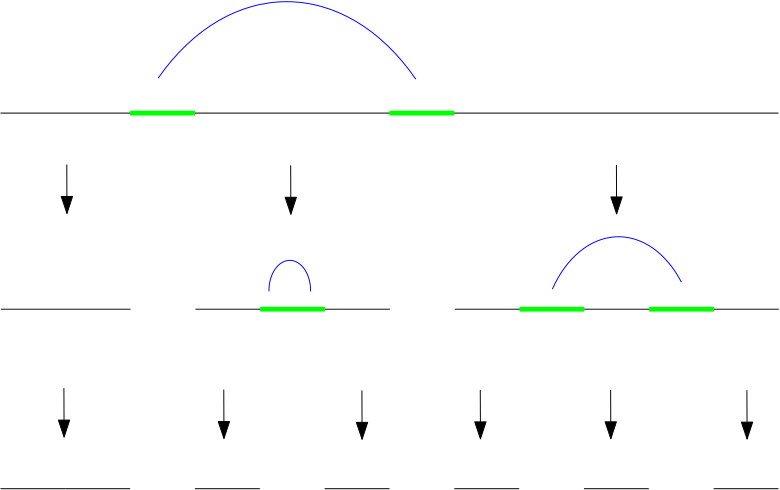
\includegraphics[scale=0.4]{images/k_local_sequence.png}
\caption{A sequence of RNA undergoing \klf. Here, we have found 3 local alignments. }
\end{figure}

\begin{algorithm}[h]
\caption{\klf}
\label{alg:klf}
\begin{algorithmic}[1]
\Procedure{k-Local Folding}{$r,k$}
\State Initialize stack $S\gets r$
\While{The number of local alignments found is $\leq k$ and $S$ not empty}
\State $s\gets \text{pop}(S)$
\State Let $\overline{s}$ be the reverse of $s$
\State Call Local Alignment on $s$ and $\overline{s}$.
\If{local alignment found}
\State Remove the aligned regions from $s$
\State Push all unmatched regions of $s$ back onto stack
\EndIf 
\EndWhile
\State Call \rf on all unmatched regions of $r$. 
\EndProcedure
\end{algorithmic}
\end{algorithm}


\subsection{Runtime Analysis}
Fix an RNA strand $r$ with length $n$. 
\begin{lemma}
Let $\al$ be the set of local alignments found. Finding $k$ disjoint local alignments of $r$ takes time $O(n^2 k)$. 
\end{lemma}
\begin{proof}
We can view the progress of the algorithm as a ternary tree: amortized across each level we perform local alignment on a sequence of size $n-\sum_{A\in\al}\ell_A$. Local alignment takes time squared in the size of the input. Since the tree in the worst case has depth $k$, the result follows. 
\end{proof}

\begin{lemma}
\klf runs in time
\[O\left(\left(n-\sum_{A\in\al}\ell_A\right)^3+n^2k\right),\] where $\ell_A$ is the length of an alignment $A\in\al$. 
\end{lemma}
\begin{proof}
Running \rf takes cubic time in the size of the input. \klf first finds $k$ disjoint alignments, then runs \rf on the remaining unmatched regions, which have total length $n-\sum_{A\in\al}\ell_A$.   The result follows by applying lemma 1. 
\end{proof}

It is worth remarking that it is very unlikely that the depth of the tree is $k$: it will more likely be $\log(k)$. Therefore, an average case analysis will yield that \klf runs in time 
\[O\left(\left(n-\sum_{A\in\al}\ell_A\right)^3+n^2\log (k)\right).\]

Now, it is clear that since $O((n-\sum_{A\in\al}\ell_A)^3)=O(n^3)$, asymptotically there is no difference between \klf and \rf. However, we will demonstrate that there is indeed a difference in practice. To illustrate this it is useful to look at two extreme cases.\\

1) Consider a perfect hairpin in which case the entire sequence of $r$ is a complementary palindrome eg $r = GGG \ldots CCC$ Smith-Waterman will match the entire strand to itself and \rf will not do any work. \\
2) Consider $r = AAA \dots AAA$ where there is no complementarity and can be no internal binding. There will be no pruning done by the preprocessing, and \rf will do its maximum amount of work. \\


At this point, it is worth reiterating that \klf is not a method intended to replace \rf. Instead, it might be used when a lower score accuracy is acceptable when an increase in speed is desired. 

\section{Results}
Experiments were run on several RNA datasets. A random set of twenty RNA strands were chosen from each set and, for each $k$, their scores and runtimes were averaged. Only the first 250 base pairs of each strand were kept, for the purposes of time. \\

The code was written in python, and can be accessed at \url{https://github.com/bchugg/bwt}.


\subsection{Runtime Comparison}
\begin{figure}[h!]
\centering
\subfloat[$k\in\{0,1,\ldots,10\}$]{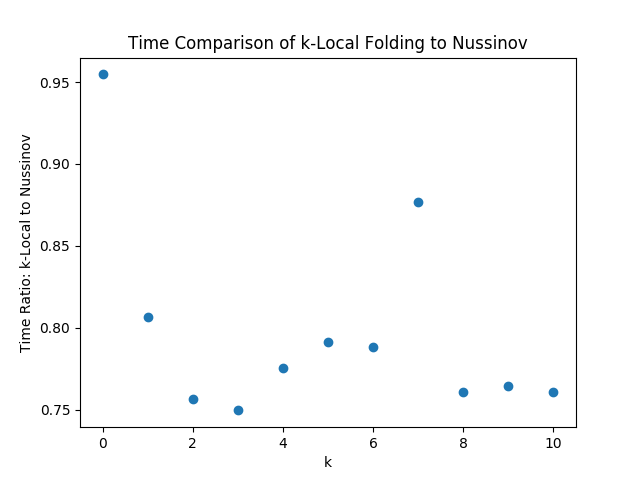
\includegraphics[scale=0.5]{../figures/TIME_k0-10_20seqs_rna.png}}
\subfloat[$k\in\{14,\ldots,20\}$]{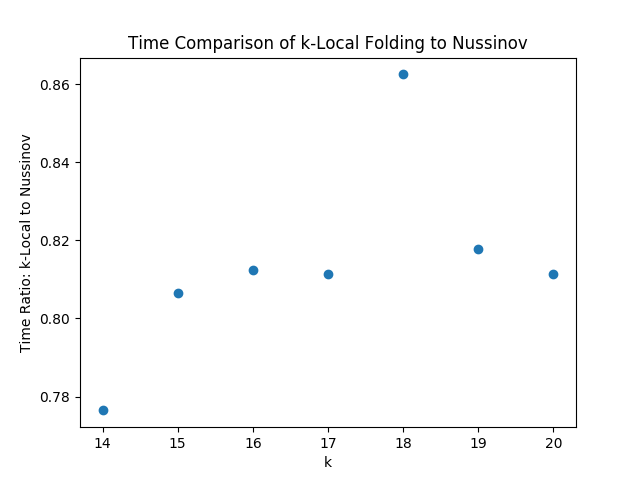
\includegraphics[scale=0.5]{../figures/TIME_k14-20_20seqs_rna.png}}
\caption{16S Ribosomal Subunit RNA}
\end{figure}
\begin{figure}[h!]
\subfloat[$k\in\{0,\ldots,10\}$]{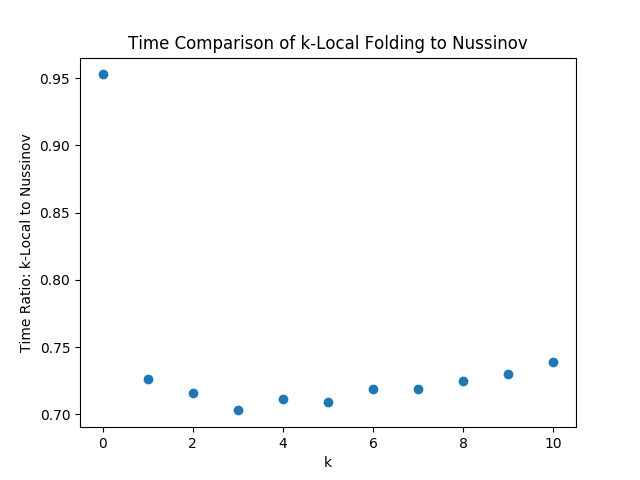
\includegraphics[scale=0.5]{../figures/TIME_k0-10_20seqs_ciliateRna.png}}
\subfloat[$k\in\{14,\ldots,20\}$]{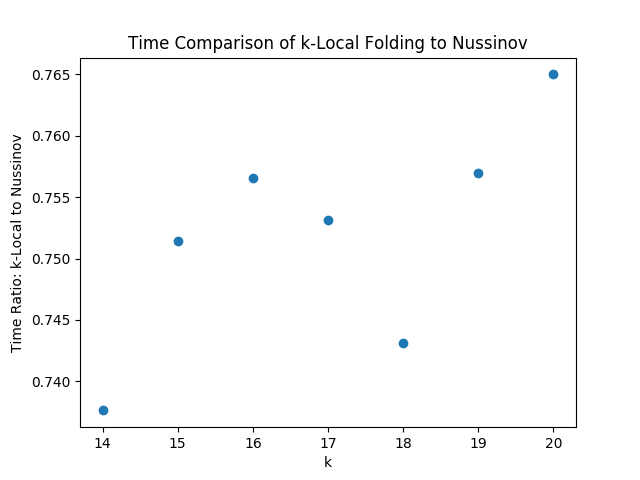
\includegraphics[scale=0.5]{../figures/TIME_k14-20_20seqs_ciliateRna.png}}
\caption{Ciliate Telomerase RNA}
\end{figure}

\newpage
For $k=0$, as expected the ratio is approximately 1:1, since \klf is not actually finding any local alignments. However, for $k>0$, we see an immediate drop in the runtime. Interestingly, for all $k>0$, there does not seem to be much difference across runtimes. Indeed, if we notice the scale of figure (b), we see that relative to figure (a) it remains almost linear. The results for both data sets look relatively similar, potentially indicating some sort of universality for the runtime of \klf. 

\subsection{Scoring Comparison}

\begin{figure}[h!]
\centering
\subfloat[$k\in\{0,1,\ldots,10\}$]{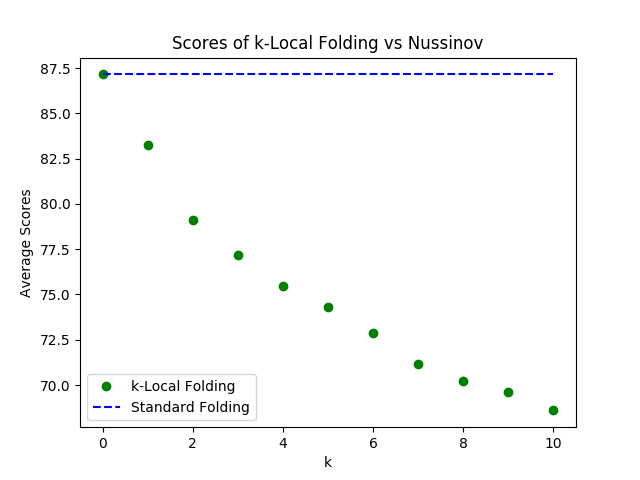
\includegraphics[scale=0.5]{../figures/SCORE_k0-10_20seqs_rna.png}}
\subfloat[$k\in\{14,\ldots,20\}$]{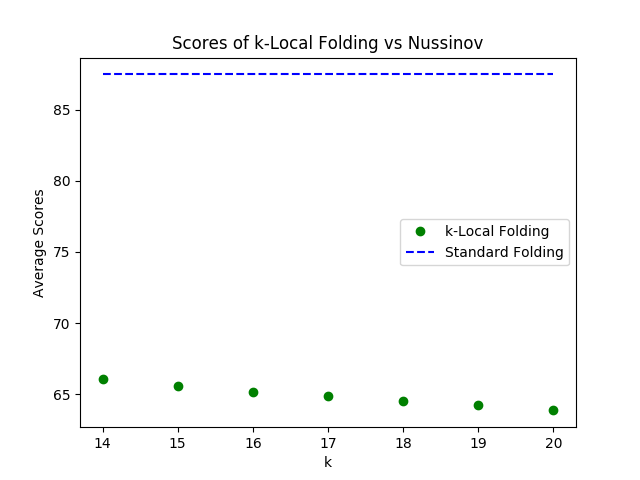
\includegraphics[scale=0.5]{../figures/SCORE_k14-20_20seqs_rna.png}}
\caption{16S Ribosomal Subunit RNA}
\end{figure}
\begin{figure}[h!]
\subfloat[$k\in\{0,\ldots,10\}$]{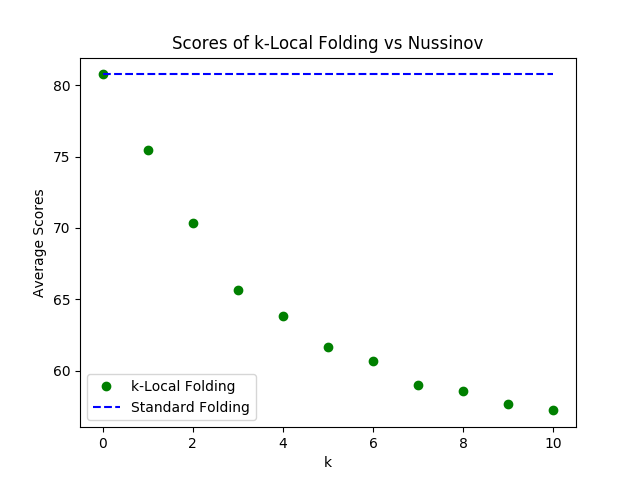
\includegraphics[scale=0.5]{../figures/SCORE_k0-10_20seqs_ciliateRna.png}}
\subfloat[$k\in\{14,\ldots,20\}$]{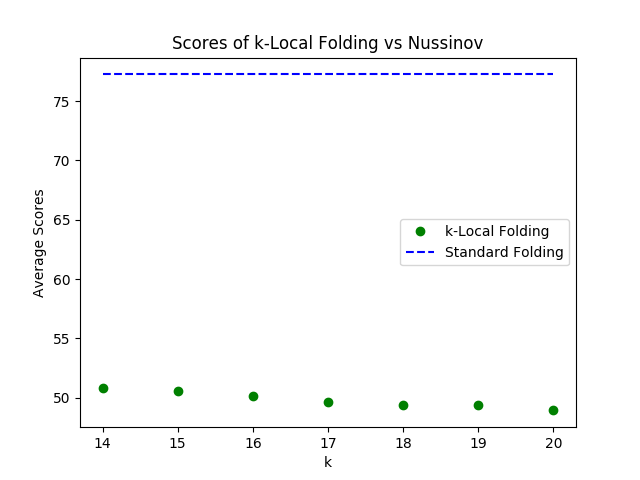
\includegraphics[scale=0.5]{../figures/SCORE_k14-20_20seqs_ciliateRna.png}}
\caption{Ciliate Telomerase RNA}
\end{figure}
\newpage

For $k=0$, the scores are identical as is expected. As $k$ increases, we see a significant decrease in the scores. This can be explained by recalling that \rf is mathemtically optimal. As we greedily align more subregions of the RNA sequence, we veer further away from the global alignment returned by \rf, hence our score decreases. This makes sense, because by choosing local alignments to pair before running \rf we constrain the possible structures reducing the search space, but likely removing the optimal structure.  

\section{Conclusion}

From the two data sets tested, it looks as though \klf does indeed beat \rf in terms of runtime. However, as $k$ increases, the score returned by \klf decreases. As such, we propose \klf as only a potential preprocessing step when an increase in speed is more important than a precise score. It is worth noting that even state of the art energy minimization models only get within about 5\% of the minimum energy, but this gap still represents potentially tens of thousands of structures, as such the divergence of scores in our approach likely corresponds to drastically different structures. However when dealing with more sophisticated energy minimization models it could also be the case that our heuristic is more likely to approach the optimal structure as these models often score contiguous runs of base pairs higher due to base stacking interactions.  


\section{Extensions and Further Research}
There are several questions which arise from this research. 
\begin{enumerate}
\item Can we decrease the runtime of \klf if we choose better data structures?

\vskip 0.25cm

For instance using a heap to store the location of where alignments start means we could run the local alignment once resulting in a run time of $O(n^{2}\log n)$ but this is worse if $k \in o(\log n)$


\item \klf can be modified to accommodate pseudoknots. 

\vskip 0.25cm

When looking for additional alignments, or when handing the remaining problems over to \rf if the segments are simply concatenated back together then this approach will find pseudoknotted structures. As $k$ increases these structures could become extremely knotted and likely are not biologically relevant. Additionally we did not explore this option so that our results were still directly comparable to \rf. 


\item Implement \klf using the Four Russians speedup for \rf and using the Burrow-Wheelers Transform to speedup Smith-Waterman.

\vskip 0.25cm

Both of these optimizations are applicable and would likely result in this approach being even faster. Additionally any other new optimizations to Smith-Waterman or \rf would also improve our technique. 

\item Can the sub-optimal alignments for \klf be found using probabilistic sampling using a Hidden Markov Model?

\vskip 0.25cm

This approach could be successful, and deserves further research. It was not addressed in this project due to lack of time and a concern that a large number of samples would be needed to find extremely short alignments. 

\item
Lower bounding the expected size of alignments found in a sequence of RNA to provide stronger guarantees about how much the problem size is reduced prior to being solved by \rf

\item 
Convert our heuristic approach to an approximation by proving bounds on how far our scores deviate from the optimal scores. 

\end{enumerate}


\bibliographystyle{plain}
\bibliography{ref.bib}


\end{document}